
\subsection{Two HOp Separated Patterns Algorithm}\label{sec:THOSPA}
We now want to focus on a specific instance of the problem stated in Algorithm \ref{alg:general}: suppose to store a graph using adjacency lists similarly to the one proposed in the Graph Join algorithm chapter (Section \vref{sec:algo}); in particular, the previous data structure is now extended with both vertex and edge containment, plus with both ingoing and outgoing edges for each single graph vertex. The latter requirement is added in order to satisfy the possibility to visit the edges backwards, thus allowing to navigate the graph in each possible direction. 
%The main data structure over which this algorithm relies  is presented in Figure \vref{nestedGraphVertex}: it shows that minor changes have been applied to the original data structure that was used to serialize graph within the graph join scenario. %Moreover, in this case we mark with different hash values the vertices within the data structure satisfying different predicates within the predicates. 
Given that the data structure requires a simple linear visit of the graph, no additional primary and secondary data structures are required. Nevertheless, during our serialization phase we provide both a primary index for accessing external informations (\textit{VertexIndex}) and the serialization of all the vertices' adjacency lists, which is going to be used for traversing the graph (\textit{VertexVals}). 
%In our straightforward implementation, hash values are here used only as placeholders for the nodes' labels used within the patterns but, given that vertices are not sorted by hash value as for graph joins, we keep the hash fields for both backward compatibility and in order to make graph joins possible for nested graphs, too.


%%Let us now restrict $\alpha$ to one single vertex and two edges: for each vertex $p_i$ matched by $\alpha$ we know that we must (possibly) visit all the edges going from $p_i$ towards the vertices $\gamma_E^{src}$ and $\gamma_E^{dst}$, that substantially are $\gamma_V$. Please note that if in $g_E$ there is no path connecting $\alpha$ to $\gamma_E^{src}$ or $\gamma_E^{dst}$, the problem may quickly become cubic with respect to the size of the vertices, because we should try to create all the possible permutations where $p_i$ is present alongside another element matching $\gamma_E^{src}$ or $\gamma_E^{dst}$. Therefore, having an edge as a constraint in $\alpha$ linking $p_i$ towards $\gamma_E^{src}$ or $\gamma_E^{dst}$ both in $g_E$ and $g_V$ can reduce all the possible computations to the actual edges traversed from $p_i$ in order to meet the grouping references, because I can reduce all the possible combinations to the ones provided by the direct graph visiting, hence possible reducing the computational complexity to the linear visit of the graph. Therefore, in this case I would know whether I finished to visit our patterns after exhaustively matching all the elements within the pattern. Even in this case, I can reduce the cost to check when I finished to traverse all the elements reaching the $\gamma_E^{src}$ and $\gamma_E^{dst}$ from $p_i$ in $\alpha$ after a linear scan of all the ingoing or outgoing nodes. Hereby, the most simple graph nesting example is where $p_i$ is the middle node between a path between $\gamma_E^{src}$ and $\gamma_E^{dst}$ vertices. 

The THoSP algorithm requires a preliminary phase, where the operand is loaded into secondary memory using the \textbf{input data  representation}, and where primary and secondary indices are serialized for backward compatibility with graph joins. Such representation is presented in Figure \ref{nestedGraphVertex}: it is an extension of the usual graph adjacency lists (\textit{\textsc{OutgoingEdges[]}}, \textit{\textsc{IngoingEdges[]}}) where each vertex $o$ has an associated \textbf{\textsc{Header}} containing its id ($o$), its associated hash and the offset pointing to other serialzied fields, such as the labelset and eventually its property-value representation ($\Braket{\ell(o),\omega(o)}$). Last, for each edge we store its id and hash value, as well as the hash and the id of the adjacent vertex. Hash values are used within the proposed THoSP algorithm to store the correspondences with the graph patterns in Figure \ref{fig:patterns}; therefore, each $\ell(o)$ is associated to a distinct hash value  $h(o)$. We also suppose that the input graph data to be serialized does not represent an exact adjacency list: for this reason, the graph is firstly created in primary memory without the offset information, and then serialized into secondary memory. 

In order to solve our specific graph nesting problem as presented in Example \vref{ex2}, we have to formally determine the $\eta$ parameters representing THoSP.
We focus on vertex (and edge) summarization patterns which grouping references associate unique vertices to distinct matching subgraphs; they require that:
\[\forall G_C\in g_V(G_o).\neg\exists G_d\in g_V(G_o).\; G_c\neq G_d\wedge f_C(\gamma_V)=f_D(\gamma_V)\]
\[\begin{split}
\forall G_C\in g_E(G_o).\neg\exists &G_d\in g_E(G_o).\; G_c\neq G_d\\
&\wedge f_C(\gamma_E^{src})=f_D(\gamma_E^{src})\wedge f_C(\gamma_E^{dst})=f_D(\gamma_E^{dst})\\
\end{split}\]
This requirement leads to a one-to-one mapping between subgraphs $G_C$ and vertices matched by vertex (or edge) grouping references, that can be expressed by the following indexing function:
\[\iota_G(G_C)=\begin{cases}
dtl(\texttt{snd}f_C(\gamma_V))_{\overline{c}} & G_C \in g_V(G_{o})\\
dtl\left(\texttt{snd}f_C(\gamma_E^{src}),\;\texttt{snd}f_C(\gamma_E^{dst})\right)_{\overline{c}} & G_C \in g_E(G_{o})\\
\end{cases}\]
This assumption permits a deterministic $\mu_E$ function, associating to each newly created nested edge from $G_C$  two nested vertices having $f_C(\gamma_E^{src})$ and $f_C(\gamma_E^{dst})$ as vertex grouping references:
\[\mu_E(G_C)=\Braket{dtl(\texttt{snd}f_C(\gamma_E^{src}))_{\overline{c}},\;dt(\texttt{snd}f_C(\gamma_E^{dst}))_{\overline{c}}}\]
Please note that the former function provides such association without additional join costs. 

\begin{figure}
\centering
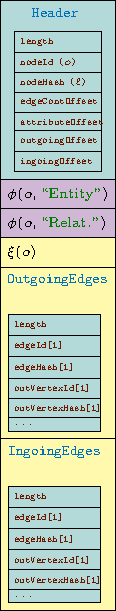
\includegraphics[height=.8\textheight]{fig/06nesting/test}
\caption{Extending the serialized graph data structure presented for graph join for the nesting operation. In particular, the present data structure extends each vertex representation in $VertexVals$ (Figure \vref{fig:graphstructure}) in order to fully supports the nested graph data model:
entities and relationships may now be contained into another data node (either a vertex or an edge). The first block of the serialized data structure contains the pointers towards the memory regions containing data which may vary in size. The fuchsia nodes remark the memory spaces where such data containments may be stored. Moreover, ingoing edges are stored as well as outgoing edges. }\label{nestedGraphVertex}
\end{figure}
\begin{algorithm}[!t]
	\caption{Two HOp Separated Patterns Algorithm (THoSP)}\label{alg:THoSPAlgorithm}
	\begin{adjustbox}{max width=\textwidth}
		\begin{minipage}{1\linewidth}
			\algrenewcommand\algorithmicindent{1em}
			\begin{algorithmic}[1]
				\Procedure{doNest}{$Index,\textsc{pattern},f, \protect\overrightarrow{memb} =\{m_1,\dots,m_n\}$}
				\For{\textbf{each} $m_i\in \protect\overrightarrow{memb}$ \textbf{s.t.} \textsc{pattern}($\protect\overrightarrow{memb}$).doSerialize($m_i$)}\label{patternrequire}
				\State{$Index$.write($\Braket{f,m_i}$)} 
				\EndFor
				\EndProcedure
				\State
				
				\Procedure{$\eta^{\texttt{false}}_{g_{V}\;,g_{E},\dots}$}{$\nested$}
				\State \textsc{File} $AdjFile$ = \textsc{Open\_MemoryMap}($\nested$);\label{openMMAP}\Comment{Serialized operand}
				\State \textsc{File} $Nesting$ = \textsc{Open}(\textbf{new}); \Comment{$\nu \cup\epsilon$, member information}
				\State \textsc{Adjacency} $toSerialize$ = \par \textbf{new} \textsc{Map<Vertex,<Edge,Vertex>>}(); \Comment{Nested graph, adj. list}
				\State {$\alpha:=V\cap {E}\backslash(\gamma_V\cup\gamma_E^{src}\cup\gamma_E^{dst})$;}\Comment{Shared pattern} \label{restriction} 
				\For{\textbf{each vertex} $v'$ in $AdjFile$}\Comment{$v':=v_c$}\label{firstJoin}
				\If{$v'\vDash\alpha$}\label{vdashalpha}
				\For {\textbf{each} $ (u',e,v')\vDash V$}\Comment{$u':=u_{c'}$} \label{substantiallyIs}
				\State{$\overline{u}:=dtl(u)_{\overline{c}}$} \Comment{$\iota_G$, nested vertex}
				\State{\textsc{doNest}($Nesting$, V, $\overline{u},\{u',e,v'\}$)}
				\For {\textbf{each} $ (w',e,v')\vDash V$}\Comment{$w':=w_{c''}$} \label{substantiallyIs2}
				\If{$ (u',e,v',e',w')\vDash E$}\label{thereIsEdge}
				\State{$\overline{w}:=dtl(w)_{\overline{c}}$}  \Comment{$\iota_G$, nested vertex}
				\State{$\overline{e}:=dtl(u,w)_{\overline{c}}$} \Comment{$\iota_G$, nested edge} 
				\State{\textsc{doNest}($Nesting$, E, $\overline{e},\{u',e,v',e',w'\}$)}
				\State{$toSerialize$.put($\overline{u}$,$\Braket{\overline{e},\overline{w}}$)}
				\EndIf
				\EndFor
				\EndFor
				\EndIf
				\EndFor
				\State $AdjFile$.serialize($toSerialize$);
				\State \Return{($AdjFile$,$Nesting$)}\label{serialize}\Comment{Nested graph}
				
				\EndProcedure
			\end{algorithmic}
		\end{minipage}
	\end{adjustbox}
\end{algorithm}
\begin{table*}[!t]
	\centering
\begin{tabular}{@{}cr|rr@{}}
	\toprule
	{\textbf{Operands' Vertices}} & Matched Graphs  & {\textbf{General Nesting} (ms)} & {\textbf{THoSP} (ms)}  \\	
	\midrule
	$10$ & $3$ &  0.57       & 0.11\\
	$10^2$ & $58$  & 0.73        & 0.14\\
	$10^3$  & $968$  & 2.78   & 0.46\\
	$10^4$ & $8,683$   & 152.11   & 4.07\\
	$10^5$ & $88,885$   & 14,015.00 & 43.81 \\
	$10^6$  & $902,020$  &  1,579,190.00      & 563.02\\
	$10^7$ & $8,991,417$   &  $>$1H      & 8,202.93\\
	$10^8$ & $89,146,891$   &  $>$1H      & 91,834.20\\
	\bottomrule
\end{tabular}
	%\end{minipage}
	\caption{Comparing the performances of the THoSP algorithm with the naive General Nesting algorithm. This comparison shows that the previously defined algorithm has a worse performance than the THoSP one. }
	\label{tab:comparisonTwo}
\end{table*}


%The main data structure over which this algorithm relies  is presented in Figure \vref{nestedGraphVertex}: it shows that minor changes have been applied to the original data structure that was used to serialize graph within the graph join scenario. %Moreover, in this case we mark with different hash values the vertices within the data structure satisfying different predicates within the predicates. 
%Given that the data structure requires a simple linear visit of the graph, no additional primary and secondary data structures are required. Nevertheless, during our serialization phase we provide both a primary index for accessing external informations (\textit{VertexIndex}) and the serialization of all the vertices' adjacency lists, which is going to be used for traversing the graph (\textit{VertexVals}). In our straightforward implementation, hash values are here used only as placeholders for the nodes' labels used within the patterns but, given that vertices are not sorted by hash value as for graph joins, we keep the hash fields for both backward compatibility and in order to make graph joins possible for nested graphs, too.
%
%Finally, Algorithm \vref{alg:THoSPAlgorithm} provides the desired implementation of the THoSP algorithm: we can observe that THoSP, contrariwise to the graph join operator, the data serialization is not included because no additional data and preprocessing steps are performed in order to provide a computational enhancement. The main memory is used to create the graph (represented as an adjacency list) that is going to be later on serialized using the same data structure used for providing the result for graph joins, that is an adjacency list where only the vertices' and edges' id appear. This choice is also done both for backward compatibility and for representing the nesting containment as a separate data structure. We can easily observe that this approach may slow down the whole algorithm, that can be quickened by directly storing the graph representation in secondary memory by using linear hashing. The nesting data structure is stored in a file as a set of pairs $\Braket{u,v}$, where $u$ represents the containing object and $v$ represents the content. By doing so, we omit the \texttt{Group By} cost which affects the previously seen query languages, thus allowing to an overall better performance. Even in this case, a join is performed between the two nested patterns: this is evident from the two nested for loops appearing in the algorithm. 

Algorithm \ref{alg:THoSPAlgorithm} provides the desired interpretation for the two pattern matching graphs returning the desired nested graph. 
%provides the desired implementation of the THoSP algorithm using the outcome of the previous preprocessing. We first restrict $\alpha$ to one single vertex and two edges 
After opening the previously-loaded graph operand through memory mapping (Line \ref{openMMAP}), we must first identify a sub-pattern $\alpha$ (Line \ref{restriction}) that is going to be visited only once within the graph (Line \ref{vdashalpha}), after which either the vertex or the path summarization pattern can be visited in their entirety. We also perform some restrictions over these patterns enhancing such optimizations: for each vertex $v'$ matched by $\alpha$ (Line \ref{vdashalpha}) we know that we must (possibly) visit all the edges going from $v'$ towards the vertices $\gamma_E^{src}$ and $\gamma_E^{dst}$.  Therefore, having an edge as a constraint in $\alpha$ linking $v$ towards $\gamma_E^{src}$ or $\gamma_E^{dst}$ both in $E$ and $V$  reduces the graph visiting time to the actual edges traversed from $v'$ meeting the grouping references (Line \ref{thereIsEdge}). Therefore, we know when we finish  our patterns' instantiation after exhaustively matching all the elements within the pattern.
As a consequence, a ``path join'' is performed between the two nested patterns (Line \ref{firstJoin} with \ref{substantiallyIs2}): this is evident from the two vertex nested for loops appearing in the algorithm.  %%We can now reduce the cost to check when we finished traversing all the elements reaching  $\gamma_E^{src}$ and $\gamma_E^{dst}$ from $v$  after a linear scan of all the ingoing or outgoing nodes. %Hereby, the most simple graph nesting example is where $v$ is the middle node between a path between $\gamma_E^{src}$ and $\gamma_E^{dst}$ vertices. 

%Even in this case, the main memory is used to create the graph (represented as an adjacency list) that is going to be later on serialized using the same data structure used for providing the result for graph joins,  We can easily observe that this approach may slow down the whole algorithm, that can be quickened by directly storing the graph representation in secondary memory by using linear hashing. 


Our physical data model differentiates the \textit{input data  represnetation} from the \textbf{query result} (Line \ref{serialize}). 
We suppose that the latter is only used by the user to read the outcome of the nesting process as in other  query languages (such as SPARQL and SQL) and does not have to
produce ``materialized views''. Therefore, the result of the graph query itself can postpone the creation of a complete ``materialized view'', which will later use the same representation of the input data by using both the id information and the application of the User Defined Functions. In particular, the former $dt$ function is used to associate both the nested vertices, $\overline{u}$ and $\overline{w}$, and the nested edge $\overline{e}$ to their grouping references, thus allowing to easily go back to the original grouping references by using the inverse function of $dt$, thus allowing the postponed application of the user defined functions.


Last, the \textsc{doNest} procedure performs the association between the nested vertices (and edges) $f$ and its members within the input graph $m_i$. When the pattern requires that $m_i$ should be a member of $f$ in the final nested graph,  \textsc{doNest} stores in a $Nesting$ file those membership associations as pairs $\Braket{f,m_i}$. By doing so, we omit the \texttt{GROUP BY} cost which affects the previously seen query languages. 


%Table \ref{tab:comparisonTwo} provides a comparison between the general Nesting Algorithm \texttt{[Should we put the previous CIKM version on arXive, so that here we just focus on the main\\ algorithm?]} and over the THoSP implementation of the query provided in our running example, under the assumptions that are going to be soon introduced in the next section. In particular, while THoSP increases linearly alongside the data size, the general nesting algorithm grows quadratically, thus quickly leading to a intractable time evaluation for big data scenarios. Hereby, the THoSP algorithm is going to be used in comparisons with other problem-specific queries on different query languages and data structures.

Please note that if in $g_E$ there is no path connecting $\alpha$ to $\gamma_E^{src}$ or $\gamma_E^{dst}$, the problem may quickly become cubic with respect to the size of the vertices, because we must create all the possible permutations where $v'$ is present alongside another element matching $\gamma_E^{src}$ or $\gamma_E^{dst}$.


Table \ref{tab:comparisonTwo} provides a comparison between the general Nesting Algorithm and over the THoSP implementation of the query provided in our running example, under the assumptions that are going to be soon introduced in the next section. In particular, while THoSP increases linearly alongside the data size, the general nesting algorithm grows quadratically, thus quickly leading to a intractable time evaluation for big data scenarios. Hereby, the THoSP algorithm is going to be used in comparisons with other problem-specific queries on different query languages and data structures.